\documentclass[]{final_report}
\usepackage{graphicx}
\usepackage{hyperref}


%%%%%%%%%%%%%%%%%%%%%%
%%% Input project details
\def\studentname{Colin Smith}
\def\projecttitle{Using RFID to Remember}
\def\supervisorname{Lorcan Coyle}
\def\moderatorname{Fintan Costello}


\begin{document}

\maketitle
%\tableofcontents\pdfbookmark[0]{Table of Contents}{toc}\newpage

%%%%%%%%%%%%%%%%%%%%%%
%%% Your Abstract here

\begin{abstract}

\textbf{\textsl{RFID has proved to be a useful technology, becoming more common with development of
applications to benefit people in everyday useful ways. This
project proposes to use this technology to aid human memory, and specifically to
help people find lost items. For most people, losing a wallet or a mobile phone is a common
occurrence. People could benefit from a system which can
help them locate lost items. Using the system is simple, it consists of an RFID component which identifies user interactions with objects. This data is used to help people locate lost items through interacting with a lost and
found application, which is based on human readable cues. For example, `The
user last took their wallet out of their bag at 12:00 along with their car keys'.
The cues are constructed based on interactions with such objects, augmented with location data, and interactions with other people. Users interact with these cues through a
web page and also receive alerts on potentially lost items, through a built in system display.}}


\end{abstract}
\newpage

%%%%%%%%%%%%%%%%%%%%%%
%%% Introduction

\chapter{Introduction}
The goal of this project is to build a system which helps users to find lost items, such as a phone or wallet. It is based on RFID technology which is used to record user interactions with these items. RFID is a way of wirelessly identifying objects, consisting of a reader and tags. When an item is tagged, it can be uniquely identified when it comes into range of the reader. Using these records of user interactions with objects, a memory aid system can be developed. This will take the form of a web site where users can obtain information about their interactions with a lost item, and aid them in remembering where they may have lost it.

The project is made up of a mobile component and a website. The mobile component consists of the RFID reader connected to a portable micro-computer. This will gather information about the users interactions such as when they had certain items and what locations and people they have come in contact with. The static component consists of a server and lost and found website. The data gathered by a portable micro computer is wirelessly
transmitted to the server, stored in a database, and presented to the
user through the website. 

This report presents a detailed overview on the progress of the project. It includes the full project specification which gives an outline of the project's specific requirements including the mandatory, discretionary and exceptional components. Chapter~\ref{background} discusses the background research required for the project. The papers presented are relevant to the technologies being used and provide useful insight into related fields of research involving these technologies. The background research also gives further insight into the applicability or usefulness of RFID for the proposed system design. Chapter~\ref{progress} gives a detailed report on work that has been completed so far. This includes objectives that have been achieved and also future milestones and work plan leading to project completion.

\section{Project Specification}

Description:
Associating interactions between users and artifacts in their everyday surroundings could be a useful way of helping people remember where they left them. When people cannot find something, simple cues like `you left your keys on the dresser table', or `i saw you take your wallet with your mobile phone' are naturally helpful. This project seeks to record a person's interactions with everyday items and generate useful cues to the user when they lose something. This project builds on an earlier ODCSSS summer school project, where an RFID reader is embedded in a glove and RFID tags are attached to kitchen implements. The reader can see when the user interacts with any item that has an attached tag and know what that item is. The earlier project recorded interactions with the kitchen implements and used them to detect when the user was completing a routine task (e.g., making a cup of tea). This project would have access to the outputs of that project and one of the challenges of this project would be to understand, reuse, and extend the earlier work.

Mandatory:
Software must be built to recognise a human user's interactions with everyday objects. These objects would be attached with RFID tags and the user will interact with them using the RFID glove. The software must be capable of giving useful (if simple) cues to remind the user where lost items are, e.g. `you interacted with your mobile phone at 2:01pm, 32 seconds after you interacted with your car keys and 21 seconds before you interacted with your wallet'

Discretionary:
A useful way for the software to communicate with the user should be developed - this might be through a lost-and-found web page, or a display attached to the glove.

Exceptional:
More complex, human readable cues should be developed, e.g., `you last had your mobile just after 2pm; you were also using your car keys and wallet at that time'.

\chapter{ Background Research}
\label{background}

\section{Introduction}

This section presents an overview of background research relevant to the project. The research papers discuss a number of relevant concepts such as ubiquitous computing, and wearable technology. These papers give a positive insight into different implementations of the proposed technologies, leading to some important conclusions on the application of RFID technology in this project.

\subsection{An Introduction to RFID Technology}

In recent years RFID has become increasingly recognised for its many potential mainstream applications and uses. There are various types of RFID available, suited to different types applications. From the highest level RFID can be divided into two classes, active and passive \cite{intel}. Active RFID requires each individual tag to have its own built in power supply. Passive RFID does not use self powered tags, they are instead charged by the reader using magnetic induction. The system being implemented for this project is based on passive RFID. Active tags would require future maintenance, such as battery replacement, and would be impractical for the projects concept. Using the passive technique the reader can power the tags and allow them to transmit a signal corresponding to its unique ID \cite{intel}.

\subsection{The Computer for the 21st Century}

Mark Weiser's seminal paper on ubiquitous computing proposes the concept of `embodied virtuality'~\cite{weiser}. He describes how in todays world information is everywhere in our environment, so much so that we do not even notice it. Technology is also a common element in our environment but it has yet to reach its full potential. He conceives a system in which computers cover free surface spaces in our surroundings, connected through an invisible network, and become part of our normal environment. One is surrounded by technology, but it vanishes into the background so as its presence is not even noted. Such a system has countless applications. The system identifies people through badges, for example, and adjusts the environment based on the individual. A person enters a room and their calls and messages are automatically transferred to them through the environment. When a person enters their place of work they are identified, at which point their office logs them in and displays documents and files, or perhaps starts to make coffee, before they have even gotten there.  An important point the author raises is that such complex systems do not require the use of complex artificial intelligence techniques. All these systems can simply be derived from simply knowing a person's location \cite{weiser}. This project proposes a similar concept. From knowing simple information about a users activities, a complex and useful application can be derived. 

\subsection{Chatchayanuson's Kitchen Tracker}

Chatchayanuson et al.'s Kitchen Tracker system proposes to aid people with grocery shopping~\cite{ece}. The system consists of stationary RFID readers in a kitchen and tags placed on key grocery items within it. As items are removed from the kitchen, i.e., used or thrown away, the RFID readers are used to identify these items. This data is used to assist in grocery shopping indicating key items that are needed in the kitchen through real time synchronisation with a phone or PDA. These implementations are based on smart home concepts \cite{ece}. One important point raised by this implementation is that such technologies should be unobtrusive and blend naturally into our environment.

\subsection {Ubiquitous Memories}

Kawamura et al.'s Ubiquitous Memories is an innovative system designed to augment human memory through interaction with objects \cite{ubi}. From a hardware perspective the system consists of a head mounted display over the left eye for displaying video to the user. This eyepiece also incorporates a camera to record user�s activities and experiences. There is an RFID reader on one wrist to read tagged objects. These are both connected to a remote control for the system which connects to a hip-mounted wearable computer. This is shown in figure~\ref{fig:borg}. This computer connects wirelessly to a LAN.
The system records the user�s experiences and activities and passes them to a server to be stored in a video database. Objects related to specific events are RFID tagged. When a tag is read the system replays a video related to that object, mimicking the behavior of human memory. When people touch objects they often recall associated memories \cite{ubi}. Ubiquitous Memories was tested using memory and recall techniques using different memory aids, one of which being the Ubiquitous Memories system. This determines the effectiveness of the system in aiding human memory and also offers insight into alternative ways of achieving this. The system is compared to other methods, in this case memory recall techniques that don't involve technology. Instead of simply rating the system performance based solely on testing it for what it is designed for, it is compared to these other methods which are designed to achieve the same goal. This knowledge could be potentially used to refine or augment the system in the future. It is this authors opinion that, like the kitchen tracker, it is important to point out that such a system needs to be unobtrusive and feel natural in our environment.

\begin{figure}[h]
\centering
\fboxsep 2mm
\framebox{
	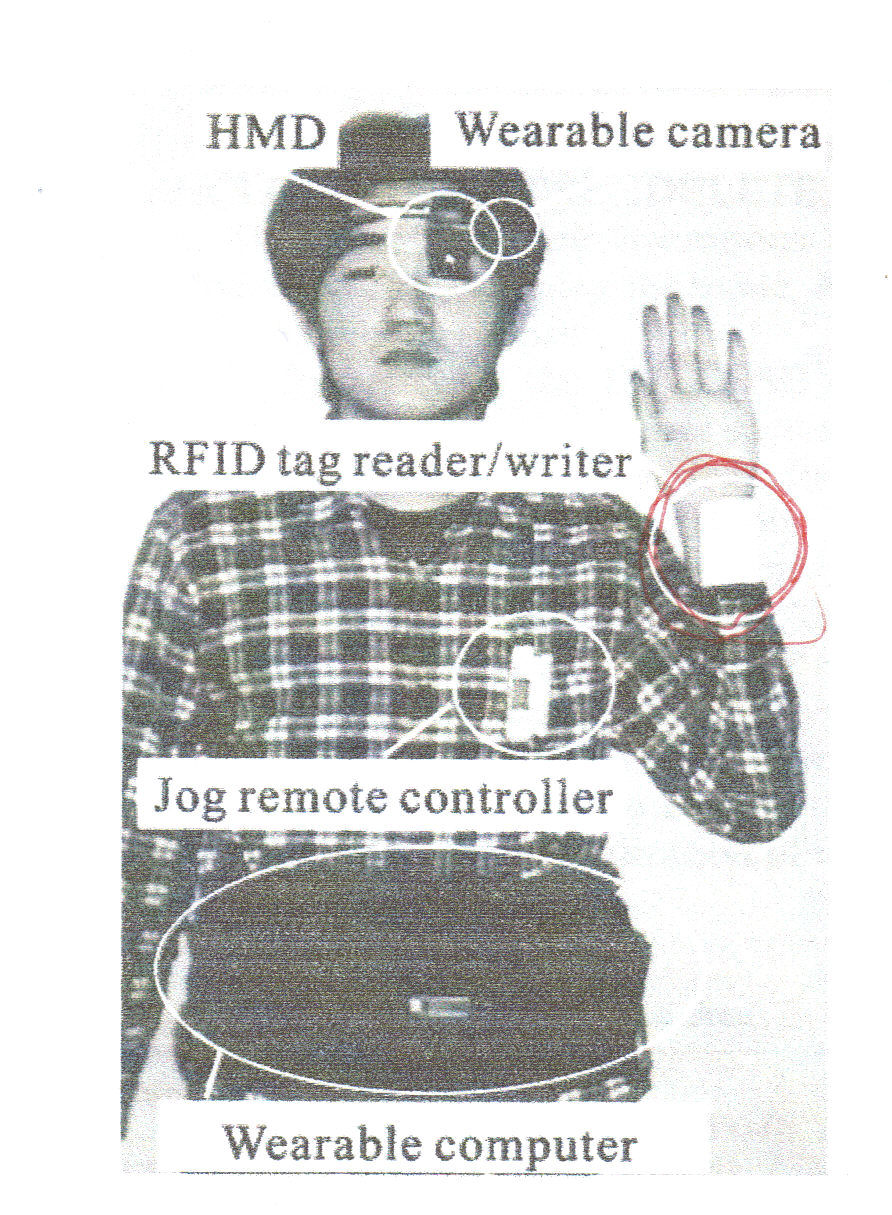
\includegraphics[width=5cm, height=7cm]{borg}
}
\caption{`Ubiquitous Memories' system}
\label{fig:borg}
\end{figure} 

\subsection {Schmidt and Gellersen's RFID glove}

Schmidt and Gellersen's RFID glove explores the area of wearable computing. In this area there is
often difficulty in providing computer input if systems carry high cognitive loads or
performance problems in their deployment \cite{schmidt}. They explore human computer interaction using an RFID based system in an attempt to overcome the
inherent shortcomings of wearable computing. The main concept is based on implicit human
computer interaction. Implicit interaction is described as actions which are not primarily
intended to be used as computer input but can still be used as such in some useful way. Their
implementation consists of a glove with an integrated RFID reader. The reader is connected
through a serial connection to a wearable computer. RFID tag IDs are mapped to a specific
URL which increases a counter each time a tag is read. They conclude that such an implementation
effectively overcomes the traditional problems associated with user input in wearable
computing, and propose that such a system would form a sound base for implementing
practical applications of the technology~\cite{schmidt}.

\subsection {Intel's iGlove}

In building useful applications with RFID technology a technique is required in order to allow
the computer to correctly interpret its inputs. Intel Seattle's iGlove research project explored the concept of recognising and interpreting an individuals activities from large sets of possibly related RFID readings. Like Schmidt and Gellersen, their system prototype was an RFID enabled glove with the antenna located in the palm. This is connected to a reader with
radio capabilities for communicating with a computer. The glove components are all housed
in a plastic box on the outer side of the glove, which overall makes the system compact and
unobtrusive, which can be seen in 
 \ref{fig:iglove}. One difficulty their system faced was interpreting `variety', for example the
same task could be completed in different ways or in a different order of steps. The proposed
solution was to represent tasks in a sequence, or probable sequence, of the objects used,
which resulted in a high level of system accuracy and performance. This is shown by their systems ability to correctly identify various tasks being undertaken by the user \cite{intel2}.

\begin{figure}[h]
\centering
\fboxsep 1mm
\framebox{
	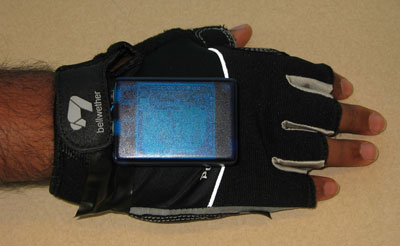
\includegraphics[width=6cm, height=4cm]{iglove} 
	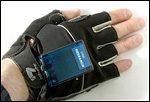
\includegraphics[width=6cm, height=4cm]{iglove2}
}
\caption{Intel's `iGlove`}
\label{fig:iglove}
\end{figure} 

\subsection {Lustig's RFID glove}

Lustig and Coyle developed a similar RFID glove system to the iGlove designed to identify
specific tasks carried out by a user \cite{cait}. A glove design was implemented with an RFID reader built into the palm, as shown in figure \ref{fig:lustig}. This
was connected to a Gumstix computer with wireless capabilities. The Gumstix can connect
wirelessly to a server which in turn can update a database of tag reads and pass this
information to a web page. The system is designed to recognise individual tasks by associating
each one with a number of relevant tags. This project extends this research
attempting to build upon the work already achieved while focusing on a related but different goal.  Although this project utilised some similar technologies, such as an RFID reader and Gumstix, the proposed project is a very different implementation and different application, the lost and found system. It will  utilise more data inputs via Bluetooth technology, and more advanced user interaction, achieved through an LCD display. Having said this it has proven useful to take into account the results and findings of their work. It was found that a glove implementation was considerably restrictive to the user, which does not conform to the principles of ubiquitous and wearable computing, which are some of the main goals of this project. This was considered a strong motivation for a new proposed form factor. 

\begin{figure}[h]
\centering
\fboxsep 2mm
\framebox{
	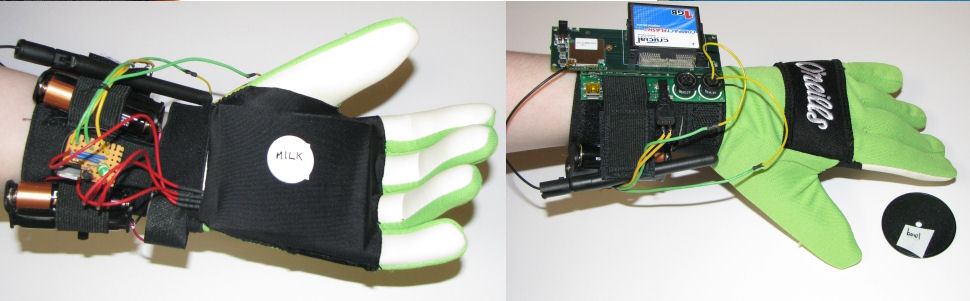
\includegraphics[width=15cm, height=4cm]{lustig}
}
\caption{Lustig and Coyle's RFID glove}
\label{fig:lustig}
\end{figure} 

\subsection{Activity Recognition}

Logan et al. explored the abilities of different sensing equipment \cite{beth}. The test system was based on a house equipped with over 900 sensor inputs, such as RFID tags, current and water flow sensors, and infrared motion detectors. The concept is similar to the iGlove and Lustig and Coyle's RFID glove, in that it uses sensor input to recognise human interactions and activities \cite{intel2, cait}. In this evaluation the effectiveness of the sensor types is discussed. In the case of RFID, the user was equipped with an RFID bracelet for reading tags in the environment, sending tag reads wirelessly to a database. The results of the experiment showed that RFID performed quite poorly. It was found that this was due to the reader detecting very few of the objects being touched. There were various reasons for this, such as opposite hands being used to interact with objects, and temporary removal of the bracelet for hygiene reasons. This raises a conflicting point to the other implementations, that RFID may not necessarily be useful in some instances. For example if a person is washing dishes they cannot have electronic equipment attached to their hands \cite{beth}.    

\subsection{Recognising Assembly Tasks}

Ward et al. explored the concept of activity recognition and ubiquitous computing \cite{jamie}. Mobile workers, such as maintenance personnel, often face difficulties in accessing useful information relevant to their task. For example a person may need to access a PDA to bring up schematics which requires complete physical and mental attention. The proposed concept involves identifying users activities and automatically display task relevant data through a head mounted display. This involves both sound and accelerometer sensors, for gesture identification, to gather data and use different algorithmic methods to identify individual tasks. The arm mounted sensors are shown in figure \ref{fig:assembly}.One problem with this, similar to that of Logan et al., involves non relevant activities \cite{beth}. For example, while a user undertakes a task they may momentarily break from this, perhaps to take something from their pocket. Their system was tested on a `mock' scenario where a user constructs a simple item from wood. Although their results were promising they conclude that their approach would be more applicable in a home environment, especially with regards to sound identification. They propose to explore other sensor and algorithmic methods, one of which being RFID, to improve the performance of the system~\cite{jamie}.
\begin{figure}[h]
\centering
\fboxsep 2mm
\framebox{
	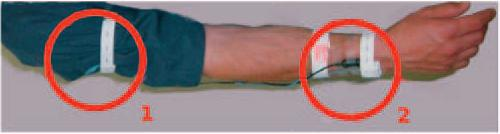
\includegraphics[width=10cm, height=3cm]{worker}
}
\caption{Arm mounted microphones and accelerometers}
\label{fig:assembly}
\end{figure}      
\section{Conclusions}
Much of this previous work in RFID applications offers some important guidance and insight for this project.
One important point raised by many of the discussed research papers is that such systems need to be
unobtrusive, feel natural to a user, and blend naturally into our environment. Ubiquitous
Memories and Chatchayanuson et al.'s kitchen tracker are good examples of this, as well as the important concept of ubiquitous computing \cite{ece, ubi}. Weiser raises another important point which is relevant to this project's system. From simply knowing some basic information, such as where you where at certain time, a more complicated and useful application can be derived, in this case a memory aid \cite{weiser}.

There are often many problems facing the concept of �wearable computing� systems, as discussed by Schmidt and
Gellerson, such as problems with performance. While this is true, it is suggested RFID offers
a sound base for implementing practical applications of these technologies and overcoming
such associated problems \cite{schmidt}. In conflict to this, Logan et al. suggested that RFID may not be useful in some instances, however their evaluation involved recognition of many, very complex user activities, over a long period of time \cite{beth}. In the instances of low performance involving RFID it seems, in this author's opinion, that the reasons for this could have been taken into account or avoided through revising and augmenting activity recognition and sensor techniques of the system. The application in this case is also quite different to that of this proposed project. Identifying a large number of complex tasks as a user undertakes their everyday home activities involves a high number of random factors, such as spontaneously switching between tasks. In the proposed system items will be static in a certain sense, where an item is placed in a pocket within very close proximity to the reader. The possibility of not reading an item in this form factor is extremely low. It can be concluded that with this systems form factor and design, RFID technology will prove very effective. 

Lustig and Coyle found their RFID system to be very restrictive
\cite{cait}. This project will explore an alternative form factor in order to overcome these
disadvantages. This project will use some of the proven hardware and technologies as Lustig and
Coyle's earlier work, but with a different implementation and application, also taking into account more useful information, such as location and interactions with other people.  

\chapter{\label{progress}Progress Report}

\section{Progress To Date}
As proposed in the project management report, the main goal of the work plan was to complete a working system by the end of January. To date a working system prototype has been completed. This consists of the mobile RFID component and the lost and found website. The mobile component consists of an RFID reader connected to a Gumstix computer~\footnote{Gumstix information can be found here: www.gumstix.com}. The Gumstix is a very small computer running a version of Linux. A circuit was constructed in order to successfully read tag ID's on the Gumstix, and to supply power to the reader. Figure~\ref{fig:circuit} shows the RFID reader connected to the Gumstix.

\begin{figure}[h]
\centering
\fboxsep 1mm
\framebox{
	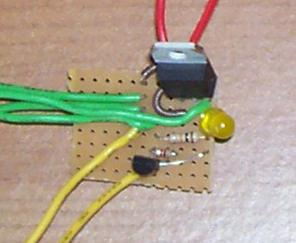
\includegraphics[width=6cm, height=6cm]{circuitShot} 
	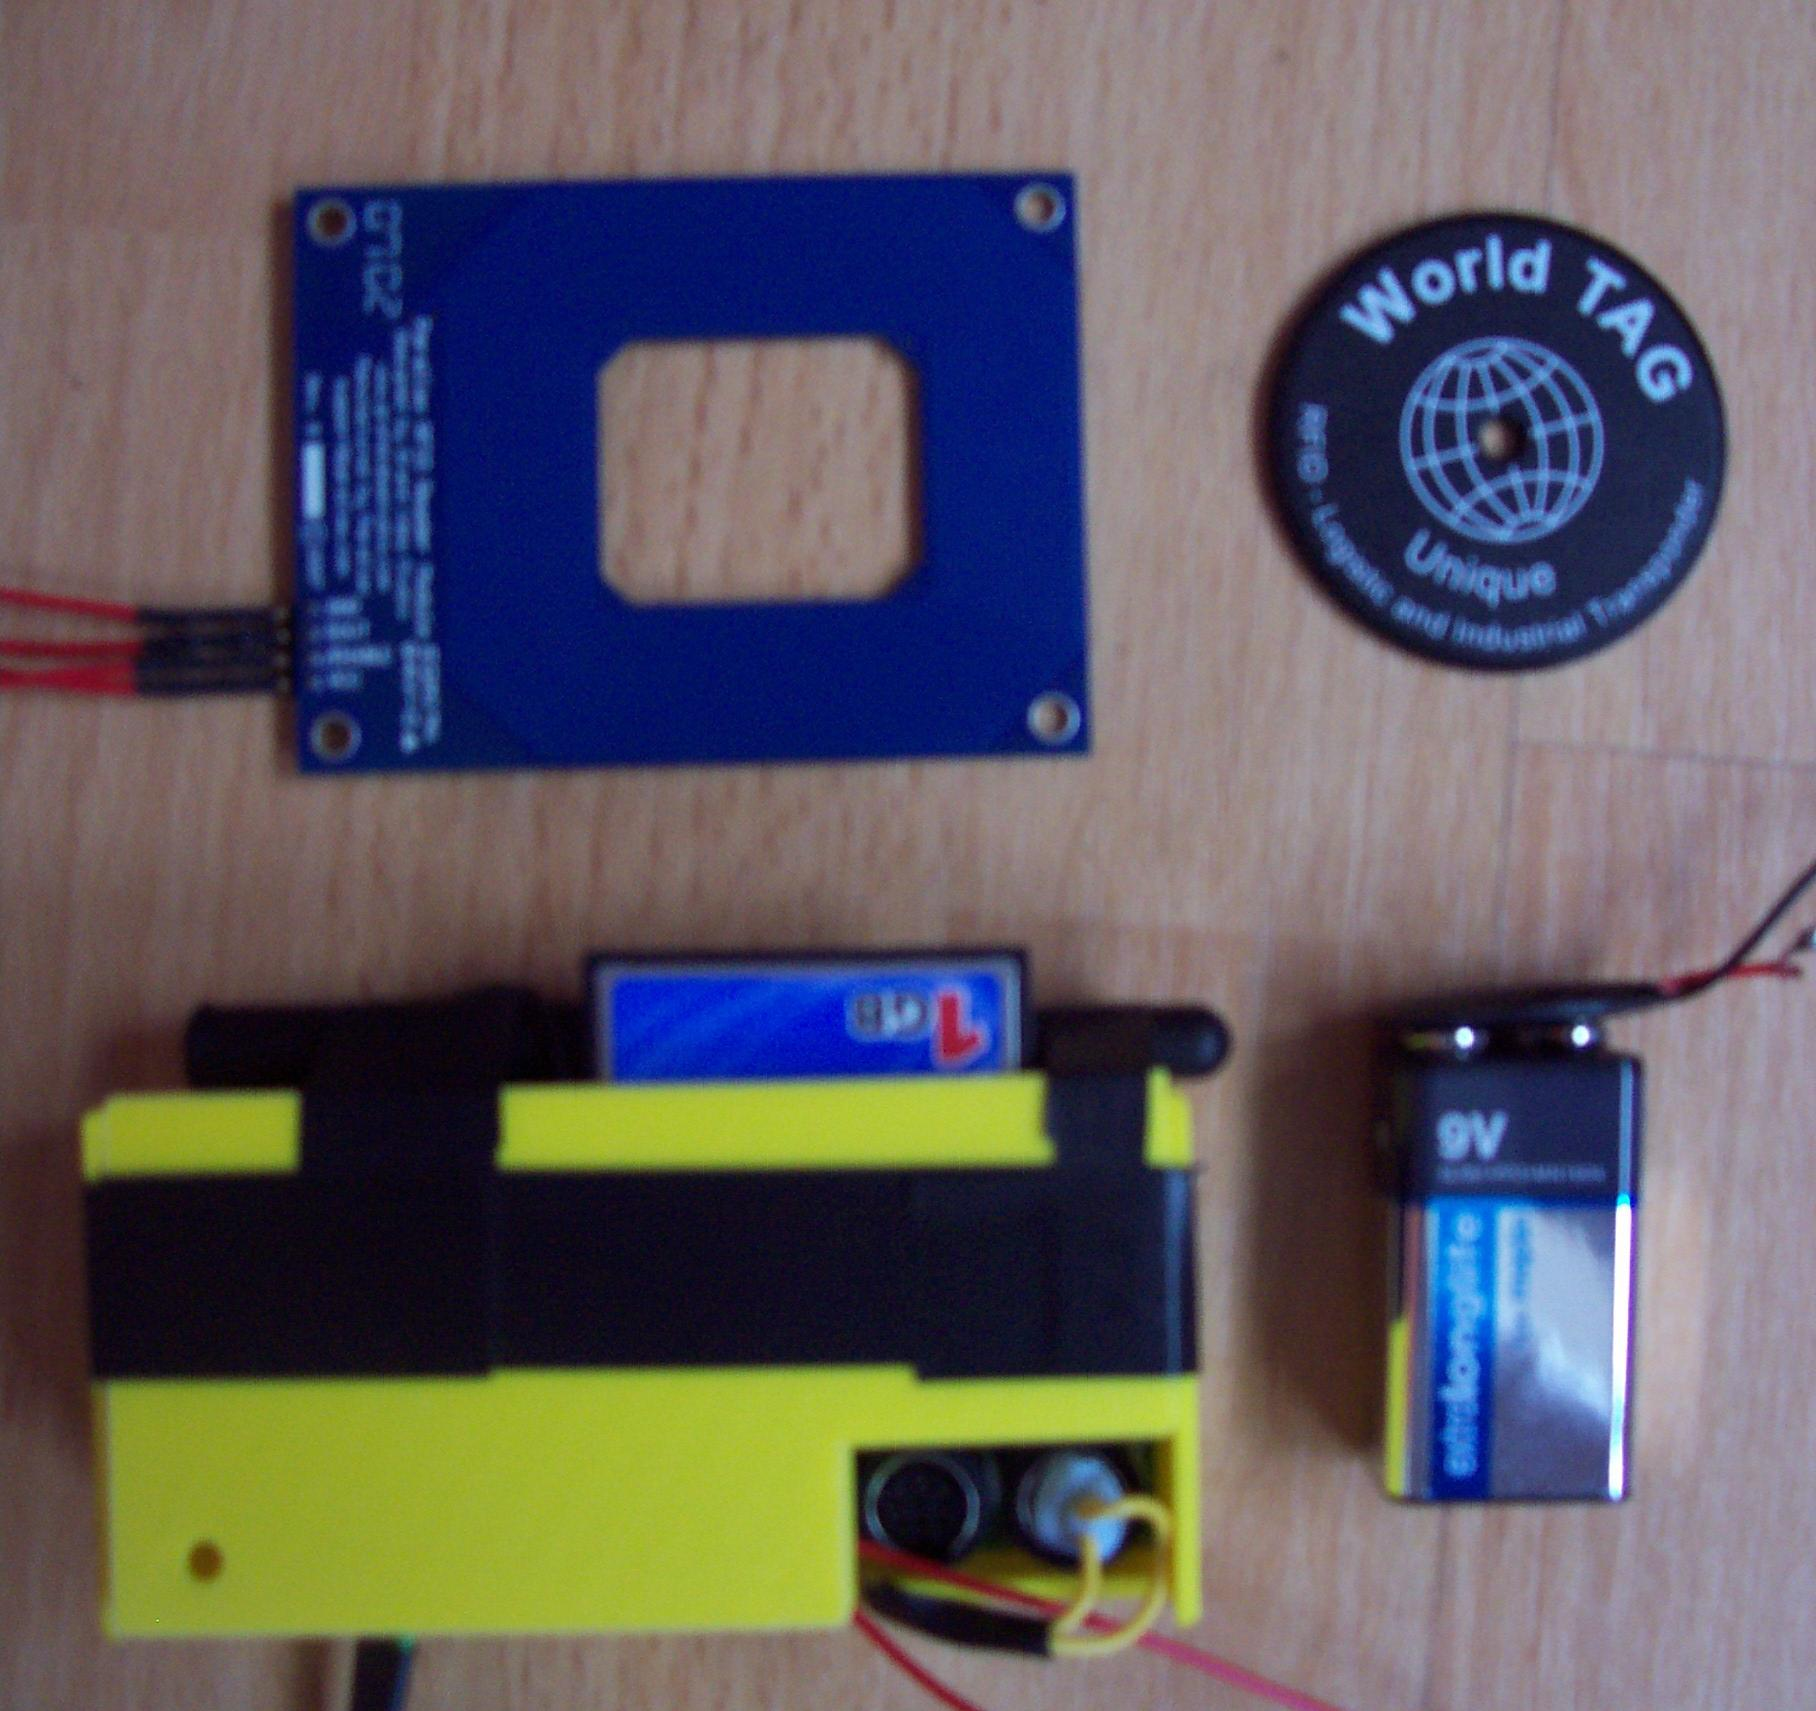
\includegraphics[width=6cm, height=6cm]{mobileShot}
}
\caption{RFID reader connected to Gumstix}
\label{fig:circuit}
\end{figure} 

A python script running on the Gumstix reads the serial port taking in these IDs. This same script is used to interact with a PHP page running on the web server. Information is transmitted wirelessly over HTTP to a database running on the server. A router was configured with internal port forwarding to serve as a wireless bridge between the Gumstix and server. A website running on the server can access tag read information in the database using PHP and MySQL~\footnote{MySQL website: www.mysql.com}. It takes this data and presents it in the form of human readable cues. If a user is looking for an item they log into the website, choose the item, and are presented with the relevant cues. Initially the cues were simple in design, displaying the item name and the last ocurrance of it in the form of a date and time stamp. Figure \ref{fig:webshot} shows a screen shot from the web site. Once the system was tested to ensure data was being read, transmitted, and stored correctly, these cues could be further developed. When a user is looking for an item the system displays when they last had it, and also checks for other items they had at this time. These cues have been made more human readable, or closer to human language, rather than simply printing timestamps, e.g., `You last had your phone just after six'. The working prototype completes the mandatory requirements for the project. The cues will continue to be improved as the system develops, taking into account more information which is discussed in the future work section. Completing these tasks in unison will result in discretionary and exceptional components being completed within the same time frame.    

\begin{figure}[h]
\centering
\fboxsep 2mm
\framebox{
	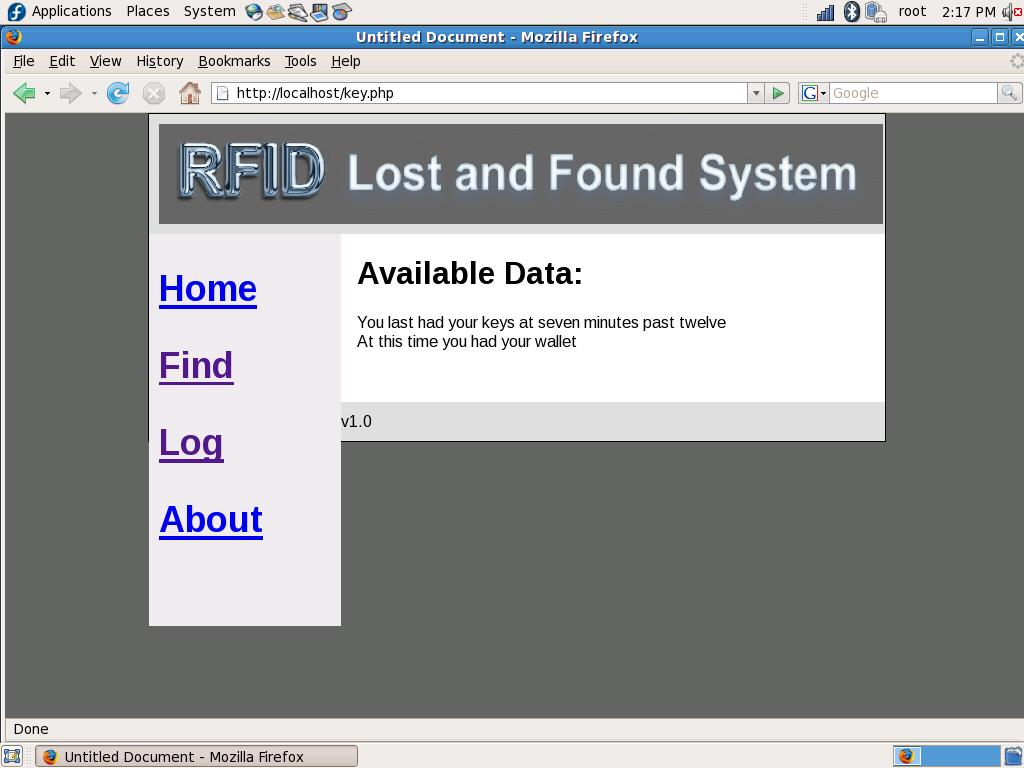
\includegraphics[width=14cm, height=9cm]{websiteShot}
}
\caption{Lost and Found website}
\label{fig:webshot}

\end{figure} 

A project wiki has been maintained in conjunction with the progress of the project. The purpose of this is to serve as a technical resource for anyone who may wish to replicate any of the different parts of the project. Continued work on this includes detailed pages on data processing and how the software is implemented. A blog has also been published~\footnote{The project blog is located at: http://colin-4thyearproject.blogspot.com/} with regular posting relating to the work that has been completed. This has proven a useful aid with regards to peer feedback and discussion of any problems that arise. Like the wiki this will also serve as a helpful resource for others wishing to replicate elements of the project.

A box was designed using a 3D printer specifically to house the Gumstix configuration being used. There is also space inside to hold the circuit connected to the RFID reader. The idea behind this is to create a compact and portable mobile component. While it is still a proof of concept, the prototype's form factor will allow it to be easily carried, such as in a jacket pocket or a bag.

As the project progresses relevant sections have been added to the final report as work is completed. Although it is still an early draft it will prove very useful when it comes to completing the final report.  

At the beginning of semester two, project supervisors organised presentations. A group of fourth year students were given the chance to present the project work they have completed to this point to a group of fourth year and PhD students. This also included a practical demonstration of the project prototypes. This was good practice for the final presentations and also gave an opportunity to get useful and constructive feedback on the system.

\section{Future Work}
Four main goals have been set to bring the project to completion. The next step will involve utilizing the Bluetooth capabilities of the Gumstix which will enable the system to scan for Bluetooth enabled devices. This will be used to identify people the user has come into contact with, based on their mobile phone Bluetooth ID. Static Bluetooth nodes will correspond to specific locations such as work and home. The goal of this is to give the user as much useful information as possible about their activities in order to help them remember where and when they may have lost an item. Combining this with the abilities of the prototype, the user will know when they last had a lost item, what other items they had at this time, what people they were in contact with, and what their location was. The next step will be to incorporate an LCD screen into the systems mobile component. This will be used to display useful information and notices to the user that they may have lost something. The user readable cues will continue to be improved ensuring they are as close as possible to human readable language. Improvements will also take into account the new data being gathered with Bluetooth, and presenting this to the user. The fourth stage will see the completion the final report and preparations for the project presentations.

The following is an outline of the proposed work plan and milestones up until project completion:
\begin{itemize}
	\item 28th March - 13th April: Complete Bluetooth component
\end{itemize}
\begin{itemize}
	\item 14th April - 1st May: Complete LCD component
\end{itemize}
\begin{itemize}
	\item 1st May - 8th May: Complete Final report
\end{itemize}
\begin{itemize}
	\item 8th May - 15th May: Presentation preparations
\end{itemize}
\begin{itemize}
	\item  The development of more human readable cues will be developed in tandem with the other components
\end{itemize}
%%%% ADD YOUR BIBLIOGRAPHY HERE
\newpage
\begin{thebibliography}{99}
\bibitem{intel}
	  Roy Want,
	  \emph{An Introduction to RFID Technology}.
	  IEEE Pervasive Computing 5, 1 (Jan. 2006), 25.
	  
	\bibitem{intel2}
	  Matthai Philipose, Kenneth P. Fishkin, Mike Perkowitz, Donald J. Patterson, Dieter Fox, Henry Kautz, and Dirk Hahnel,
	  \emph{Inferring Activities from Interactions with Objects}.
	  IEEE Pervasive Computing 3, 4 (Oct. 2004), 50-57.  
	  
	  \bibitem{ece}
	  Suppakrit Chatchayanuson, Charles Christopher Oneyama, Nachiket Shelgikar, Saravana Sivasankaran 
	  \emph{Kitchen Tracker}.
	  Electrical and Computer Engineering, Carnagie Mellon University, 2007.
	  
	  \bibitem{ubi}
	  Tatsuyuki Kawamura, Tomohiro Fukuhara, Hideaki Takeda, Yasuyuki Kono, and Masatsugu Kidode 
	  \emph{Ubiquitous Memories: a memory externalization system using physical objects}.
	  Personal Ubiquitous Comput. 11, 4 (Apr. 2007), 287-298. 
	  
	  \bibitem{smart}
	  Alex S. Taylor, Richard Harper, Laurel Swan, Shahram Izadi, Abigail Sellen, and Mark Perry
	  \emph{Homes that make us Smart}.
	  Personal Ubiquitous Comput. 11, 5 (Jun. 2007), 383-393.  
	  
	  \bibitem{cait}
	  Caitlin Lustig, Lorcan Coyle
	  \emph{Reminding Short-Term Memory Sufferers to Complete Routine Tasks}.
	  Technical Report UCD-CSI-2007-10, 2007
	  
	  \bibitem{schmidt}
	  A. Schmidt and C. M. Hans-W. Gellerson
	  \emph{Enabling implicit human computer interaction- a wearable rfid-tag reader}.
	  Proc. 4th Int'l Symp. Wearable Computers (ISWC2000), pp. 193-194
	  
	  \bibitem{weiser}
	  Mark Weiser
	  \emph{The Computer for the 21st Century}.
	  SIGMOBILE Mob. Comput. Commun. Rev. 3, 3 (Jul. 1999), 3-11.
	  
	  \bibitem{beth}
	  Beth Logan, Jennifer Healey, Matthai Philipose, Emmanuel Munguia Tapia, Stephen S. Intille
	  \emph{A Long-Term Evaluation of Sensing Modalities for Activity Recognition}.
	  Ubicomp 2007: 483-500 
	  
	  \bibitem{jamie}
	  Jamie A. Ward, Paul Lukowicz, Gerhard Tr�ster, Thad Starner
	  \emph{Activity Recognition of Assembly Tasks Using Body-Worn Microphones and Accelerometers}.
	  IEEE Trans. Pattern Anal. Mach. Intell. 28(10): 1553-1567 (2006)
	  
\end{thebibliography}
\label{endpage}



\end{document}

\end{article}
